Uno de los ejercicios de examen será identificar los componentes de una imagen de una máquina (PC, Pórtatil).

Cada uno de los portátiles tiene un formato propio.

Se proporciona información sobre los componentes de la placa base, en especial, en los manuales de Prado.

En cuanto al montaje de los componentes de la placa base, debemos de tener cuidado:
\begin{itemize}
    \item Que esté apagado.
    \item Debemos de usar guantes que no conducen la electricidad, aunque en los actuales, suelen estar protegidos.
    \item No tocar nada metálico con la placa base.
    \item Un componente solo se instala de una manera, no debemos de forzarlo.
\end{itemize}

\subsection{Fuente de Alimentación}

Suele ser la parte que más se avería. Se puede comprobar con un polímetro. La fuente de alimentación posee numerosos puertos para cargar cada una de las partes de la máquina que requieren enegía.

Hay varios tipos de fuentes de alimentación.

Otra de las partes es el módulo regular de voltaje, esta pensado para evitar que el ordenador se pueda quemar, entre otras palabras.

En cuanto a los procesadores, hay dos tipos:
\begin{itemize}
    \item PGA.
    \item LGA.  
\end{itemize}


\begin{tcolorbox}[colback=yellow!5!white,colframe=yellow!75!black]
    \textbf{Pregunta de examen:} ¿Un conector de tipo PGA tiene pines alargados (patillas) que se enganchan al procesador? \textbf{Verdadero o Falso} Es falso.
    
\end{tcolorbox}

\begin{figure}[H]
    \centering
    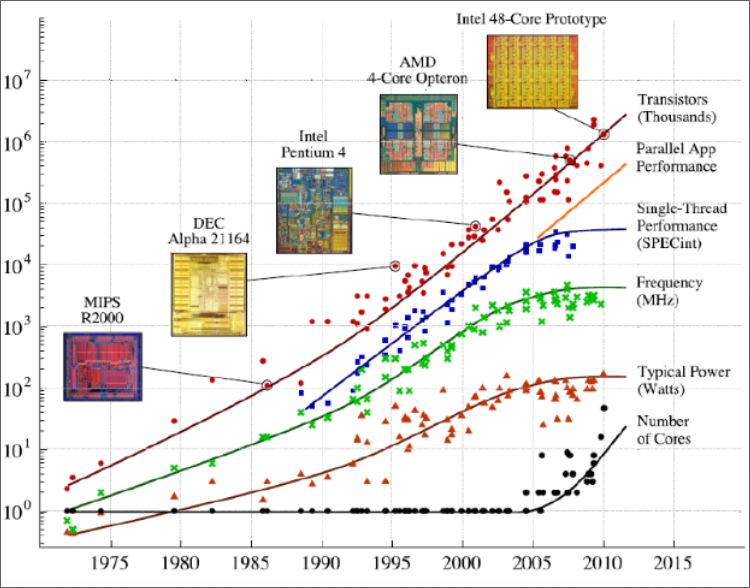
\includegraphics[width=0.8\textwidth]{images/Tema2/evol.png}
    \caption{Evolución histórica de los microprocesadores.}
    \label{fig:1}
\end{figure}

\textbf{Preguntas de examen:}
\begin{itemize}
    \item ¿Que pasó en 2005 relacionado con la frecuencia de los procesadores?. Responder en base a la imagen de arriba. Que deciden poner más cores,\dots
    \item ¿Que diferencia a un procesador de sobremesa a uno de servidores? Número de cores.
    \item Diferencias enter un microprocesador de PC a los de servidores (Transparencia número 15).
    \item ¿Que es un canal de RAM? Conecta la memoria con el procesador, de manera que se puede leer más rápido.
\end{itemize}

Un servidor tiene instrucciones distintas a las de ordenadores de sobremesa, debido a que estan destinados por ejemplo a virtualización de máquinas virtuales.

Los procesadores AMD para servidores, son multichips, es decir, tienen varios procesadores en un mismo chip (no todos).

Otra pregunta:
¿La primera arquitectura de 64 bits fue en 2004? Falso, ya había en los años 90.

Otra de las partes de un ordenador que podemos destacar es el \textit{IBM POWER}, que significa Performance Optimization With Enhanced RISC.

Luego podemos encontrar el disipador de calor, que se encarga de refrigerar el procesador.

Tenemos ranuras de memoria DRAM (Dynamic RAM), que es donde se conecta los módulos de memoria principal. Dentro del procesador hay memoria RAM, pero es estática. La memoria RAM es volátil, es decir, que si se apaga el ordenador, se pierde la información.

\begin{figure}
    \centering
    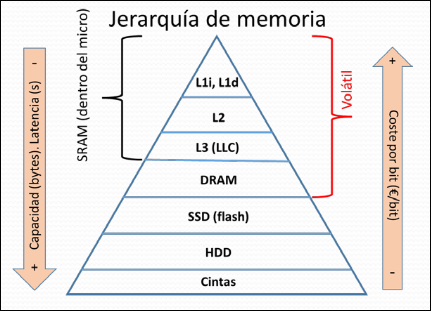
\includegraphics[width=0.8\textwidth]{images/Tema2/piramide.png}
    \caption{Jerarquía de memoria.}
    \label{fig:2}
\end{figure}
Las cintas de la imagen, se usan para copias de seguridad, ya que son muy lentas.

En cuanto a la evolución histórica de la memoria RAM, podemos destacar que primero estaba la DRAM, luego surge la PM, luego la SDRAM,\dots

Al principio tenían lo que conocemos como 'patitas', luego pasan a conectores, y luego a conectores que se encuentran por delante y por detrás.

Tenemos diversos tipos de DMIM (Dual Data Rate Inline Memory Module), que son módulos de memoria RAM:
\begin{itemize}
    \item Para servidores.
    \begin{itemize}
        \item EU-DIMM. U-DDIM con corrección de errores. Por cada línea\footnote{Como línea nos referimos a las líneas de datos, de manera gráfica ver la diapositiva 23, líneas con números en ECC RAM.} de datos se pasan 8 bits de corrección de errores y otros 8 bits de datos.
        \item R-DIMM: Registered DIMM. Hay un registro que almacena
        las señales de control (operación a realizar, líneas de
        dirección…). Mayor latencia que EU-DIMM pero permiten
        módulos de mayor tamaño. Tienen ECC.
        \item LR-DIMM: Load Reduced DIMM. Hay un buffer que
        almacena tanto las señales de control como los datos a
        leer/escribir. Mayor latencia que R-DIMM, pero son las que
        permiten los módulos con mayor tamaño. Tienen ECC
    \end{itemize}
    \item Para PC y portátiles.
    \begin{itemize}
        \item DIMM: Unbuffered (ó Unregistered) DIMM.
        \item SO-DIMM. Small Outline DIMM. Tamaño más reducido para
        equipos portátiles (tienen menos contactos).
    \end{itemize}
\end{itemize}

Cuando se aumenta el número de pines es más eficiente. En cuanto al ancho de banda debemps de tener en cuenta que va aumentando también. En la diapositiva 21, no debemos de aprendernos los números, pero si debemos de saber ocmo crecen y demás.

Un procesador accede a los módulos de memoria DRAM a  través de los \textit{canales de memoria}. Debemos de tener en cuenta que cuando las encajamos no debemos de hacer mucha fuerza. Algunos módulos tienes disipadores de calor, chips,... Hay un espacio entre las memorias para que se refrigere. En cada instante de lectura no se puede leer de manera simultánea, sino que se lee de manera secuencial. Podemos distinguir entre \textit{bancos}(leemos solo de uno) y entre \textit{canales}(leemos de todos los canales a la vez), cuando son canales podemos leer al final solo de un módulo de memoria (Diapositiva 23).

El concepto de rango se refiere al hecho de tener bancos de memoria. En cuanto a la notación de $1R\times8$ se refiere a que es un módulo de memoria con un rango, y que tiene 8 chips de memoria, por lo que lee de 8 chips a la vez. (A nivel de módulo, banco es a nivel de zócalo).

Se puede dar el caso que sea Double Sided, pero 1 rank, por lo que aunque tenga rangos por delante y por detrás, solo puede leer de uno a la vez.







